\documentclass[12pt, a4paper]{article}

\usepackage{graphicx}
\usepackage{fullpage}
\usepackage{siunitx}
\usepackage{lmodern}
\usepackage[utf8]{inputenc}
\usepackage[T1]{fontenc}
\usepackage{hyperref}

\begin{document}
\title{FYSS360 Numerical exercise}
\author{Sakari Kapanen}
\date{\today}
\maketitle

A single particle electron model was used to numerically estimate the loss cone of electrons in an ECR ion source. It is also a demonstration of the confinement of electrons (and ions) in a magnetic bottle formed by the generated solenoid and hexapole magnetic fields. The simulation was implemented~\cite{code} in \textsc{C++}.

The on-axis solenoid field $B_z(r=0, z)$ and the hexapole field $\mathbf{B}(x, y)$ as defined in~\cite{instr} were plotted (figures~\ref{fig:solenoidb} and~\ref{fig:hexapoleb}).
\begin{figure}[h]
    \centering
    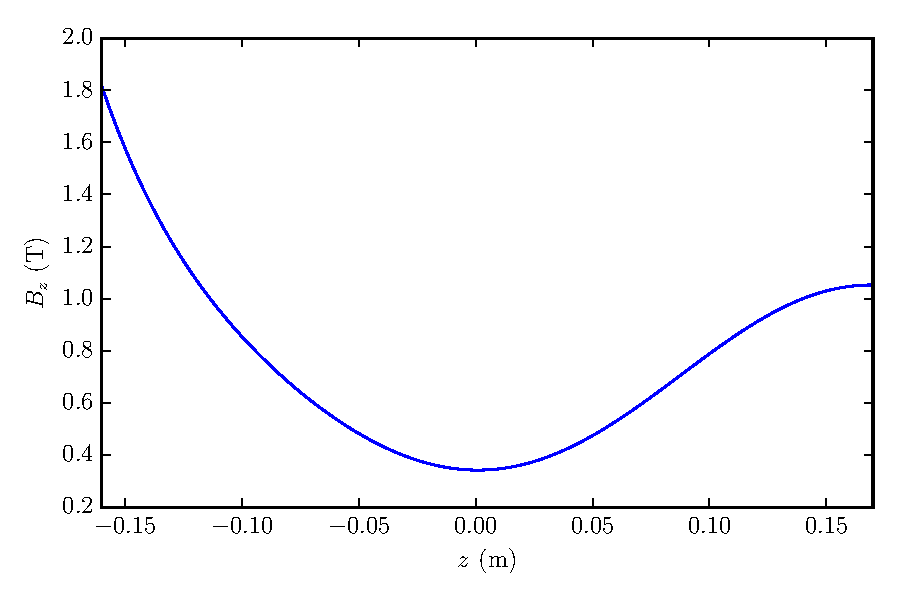
\includegraphics{output/solenoid_B_onaxis.pdf}
    \caption{Solenoid on-axis magnetic field $B_z(r=0, z)$.}
    \label{fig:solenoidb}
\end{figure}
\begin{figure}[h]
    \centering
    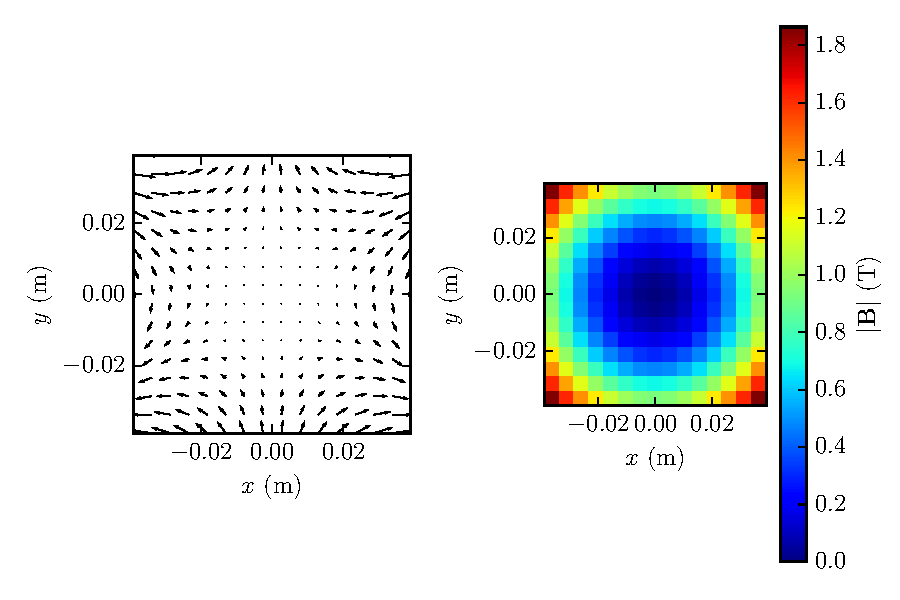
\includegraphics{output/hexapole_B.pdf}
    \caption{The direction and magitude of the hexapole B field.}
    \label{fig:hexapoleb}
\end{figure}
Slices of the total magnetic field were plotted as well at $(x=0, y, z)$ and $(x, y=0, z)$ (figures~\ref{fig:totalb_yz} and~\ref{fig:totalb_xz}).
\begin{figure}[h]
    \centering
    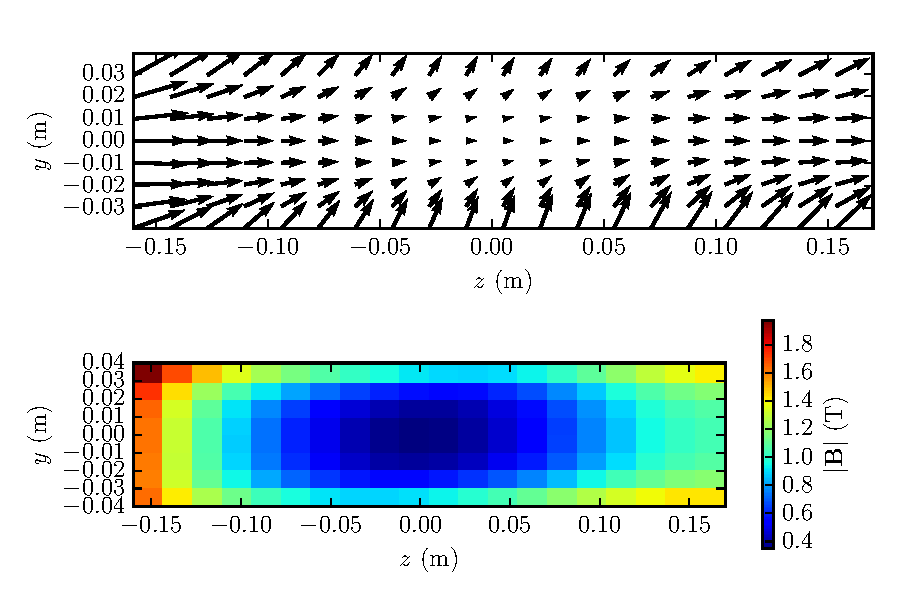
\includegraphics{output/total_B_yz.pdf}
    \caption{A slice of the total magnetic field $\mathbf{B}(x=0, y, z)$. }
    \label{fig:totalb_yz}
\end{figure}
\begin{figure}[h]
    \centering
    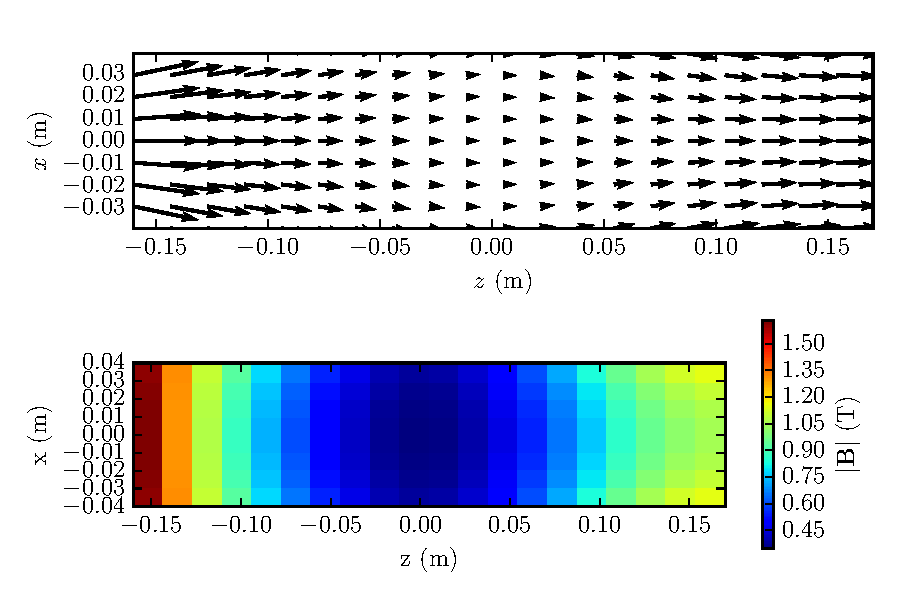
\includegraphics{output/total_B_xz.pdf}
    \caption{A slice of the total magnetic field $\mathbf{B}(x, y = 0, z)$. }
    \label{fig:totalb_xz}
\end{figure}

Electrons with uniform random velocities (with constant energy $10\,\si{\kilo\electronvolt}$) and positions inside the cylindrical plasma chamber ($z_1 = -160\,\si{\milli\meter}$, $z_2 = 170\,\si{\milli\meter}$ and $r = 39\,\si{\milli\meter}$) were generated. Further selection was done with respect to the position: only electrons with position $\mathbf{r}$ such that $|\mathbf{B}(\mathbf{r})| < 0.5\,\si{\tesla}$ were accepted for the simulation --- these correspond to electrons within the ECR zone.

The paths of the electrons were tracked independently, one at a time. The Boris integrator was used to solve the equations of motion in the presence of a static magnetic field. In order to determine the timestep length sufficient to maintain stability, the trajectory of one random particle was tracked for $10^{-8}\,\si{\second}$ and plotted with timestep lengths $10^{-10}$, $10^{-11}$ and $10^{-12}\,\si{\second}$ (figures~\ref{fig:particle10},~\ref{fig:particle11} and~\ref{fig:particle12} respectively).
\begin{figure}[t]
    \centering
    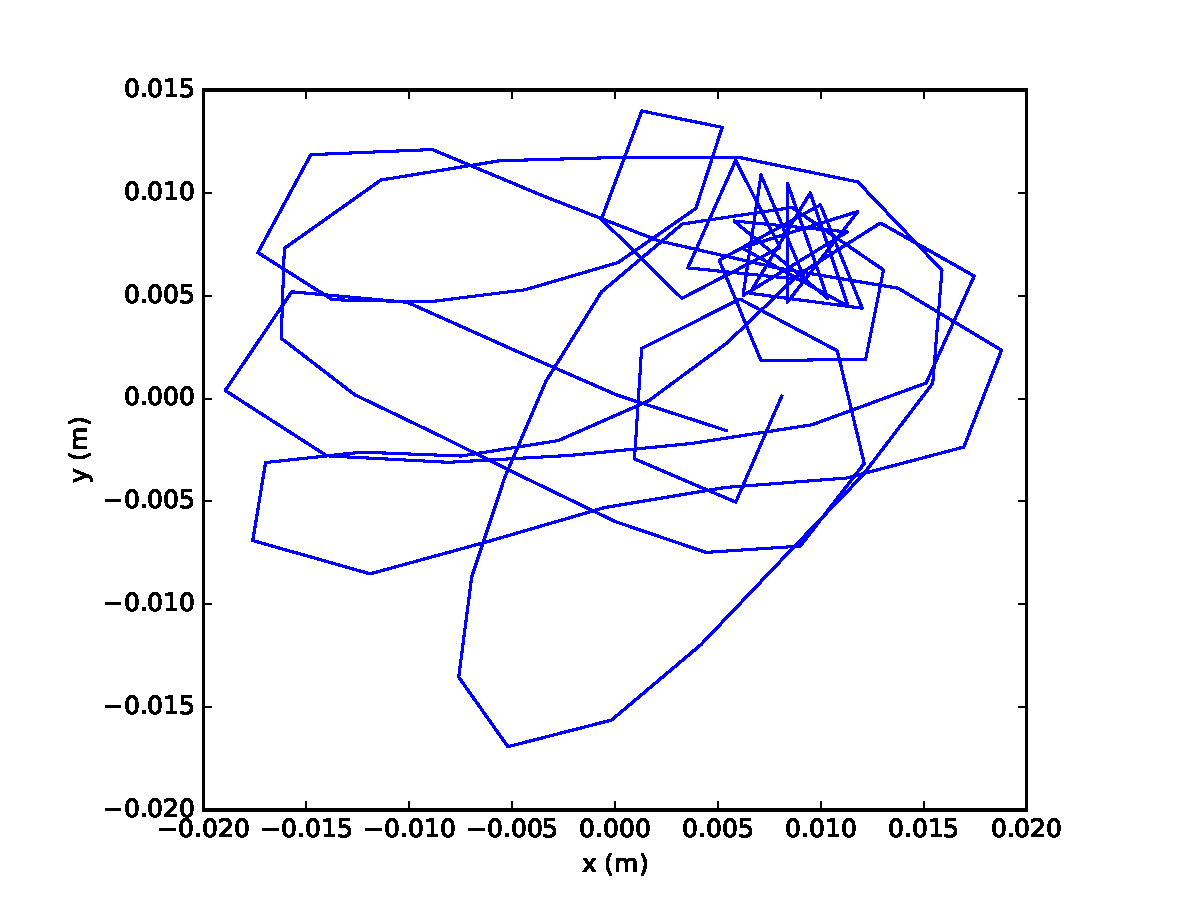
\includegraphics{output/particle_trajectory_10.pdf}
    \caption{The trajectory of a particle with timestep $\Delta t = 10^{-10}\,\si{\second}$.}
    \label{fig:particle10}
\end{figure}
\begin{figure}[t]
    \centering
    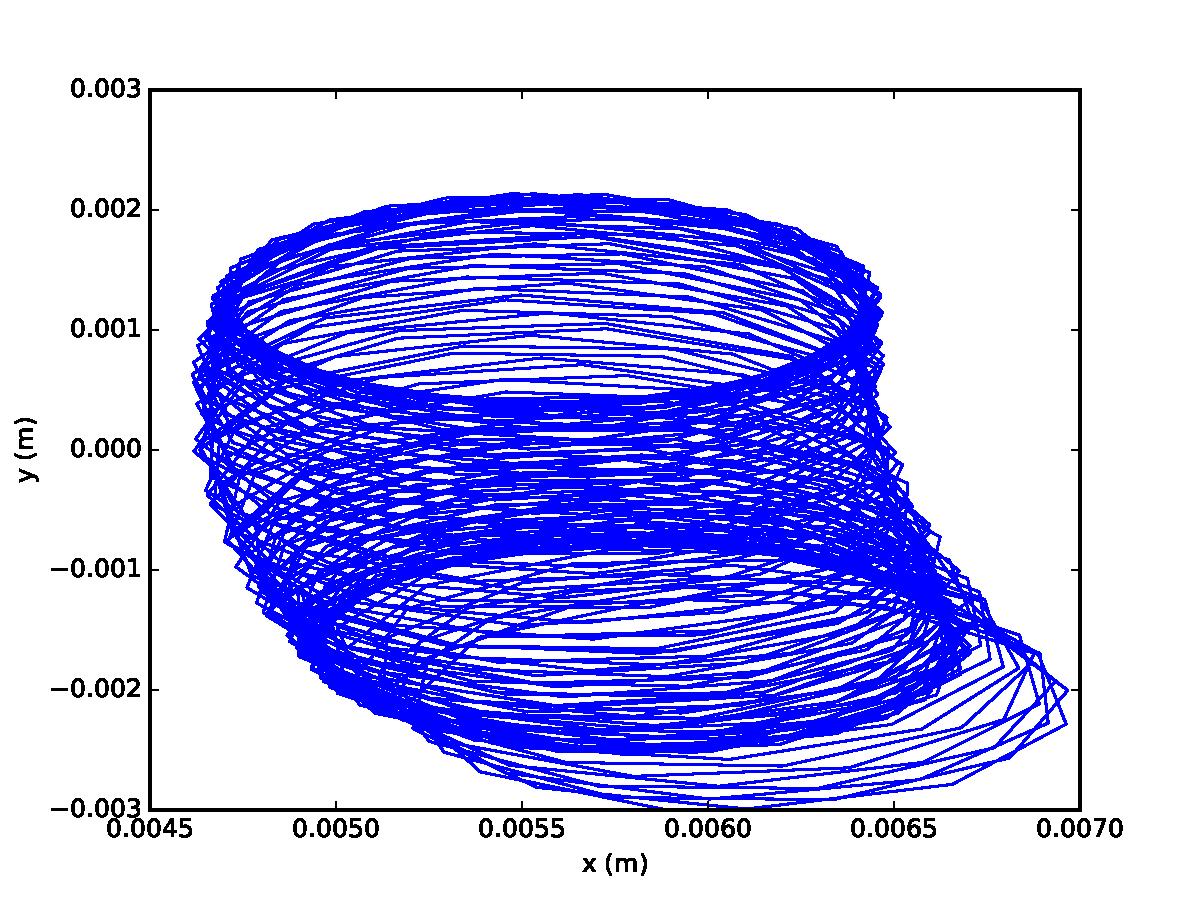
\includegraphics{output/particle_trajectory_11.pdf}
    \caption{The trajectory of a particle with timestep $\Delta t = 10^{-11}\,\si{\second}$.}
    \label{fig:particle11}
\end{figure}
\begin{figure}[t]
    \centering
    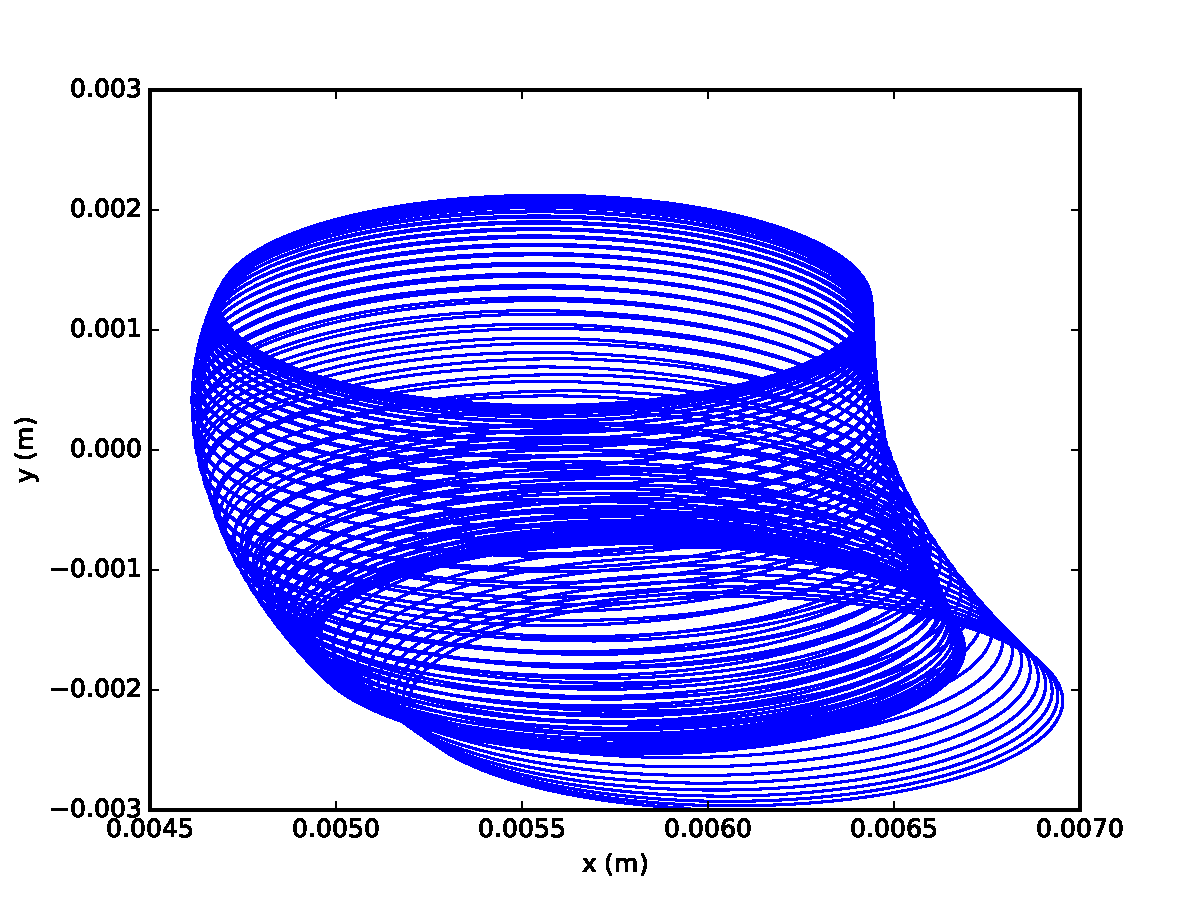
\includegraphics{output/particle_trajectory_12.pdf}
    \caption{The trajectory of a particle with timestep $\Delta t = 10^{-12}\,\si{\second}$.}
    \label{fig:particle12}
\end{figure}
From these figures it is immediately seen that at $\Delta t = 10^{-10}\,\si{\second}$ the solution is unstable. At $\Delta t = 10^{-11}\,\si{\second}$ it seems that for this trajectory stability is achieved. In the end, a timestep length $\Delta t = 5\times 10^{12}\,\si{\second}$ was chosen. This is in good correspondence with the stability limit of the leapfrog method:
\begin{equation}
    \Delta t \leq \frac{2}{\omega} = \frac{2 m_\text{e}}{eB_\text{ECR}} \approx 2.3\times 10^{11}\,\si{\second},
\end{equation}
where the electron gyration frequency due to the magnetic field at the ECR surface, $B_\text{ECR} = 0.5\,\si{\tesla}$ was substituted. It also leaves some room for larger $B$ field magnitudes but is not unnecessarily small.

In order to have sufficient statistics, the number of test particles was chosen to be $N=10^5$. Particles were tracked until they hit any of the cylinder ends and walls or the confinement time of $10^{-6}\,\si{\second}$ was elapsed. The locations where the electrons hit the geometry were recorded. Histograms for the end circles at $z_1 = -160\,\si{\milli\meter}$ and $z_2 = 170\,\si{\milli\meter}$ and the radial wall are shown in figures~\ref{fig:z_1_coll},~\ref{fig:z_2_coll} and~\ref{fig:wall} respectively.
\begin{figure}
    \centering
    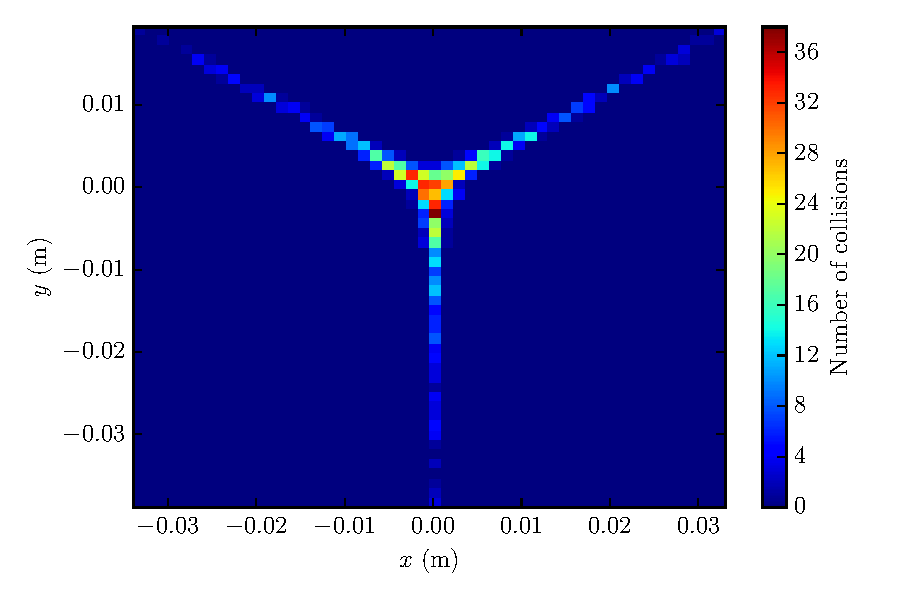
\includegraphics{output/z1_collision_points.pdf}
    \caption{Histogram of electron collision locations at the end circle $z_1=-160\,\si{\milli\meter}$.}
    \label{fig:z_1_coll}
\end{figure}
\begin{figure}
    \centering
    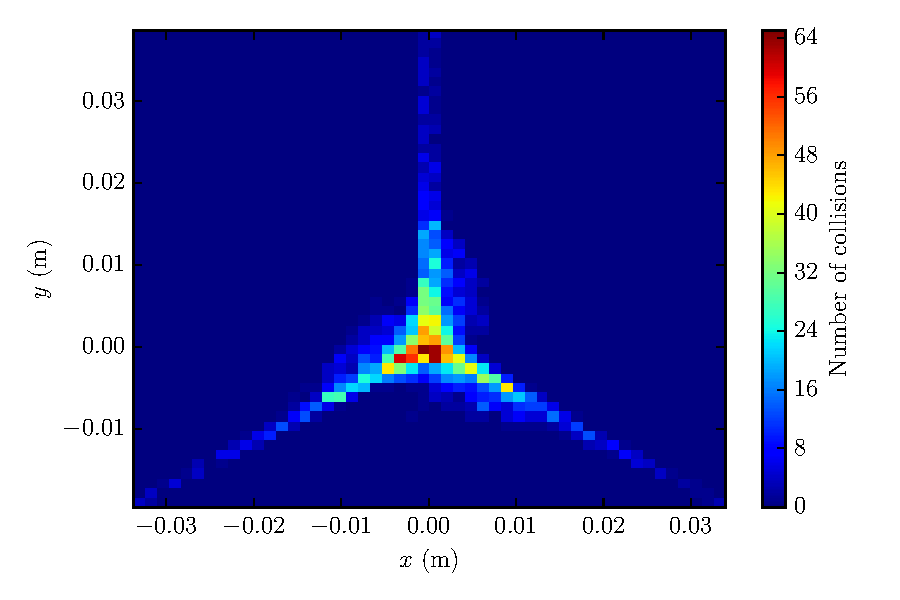
\includegraphics{output/z2_collision_points.pdf}
    \caption{Histogram of electron collision locations at the end circle $z_2=170\,\si{\milli\meter}$.}
    \label{fig:z_2_coll}
\end{figure}
\begin{figure}
    \centering
    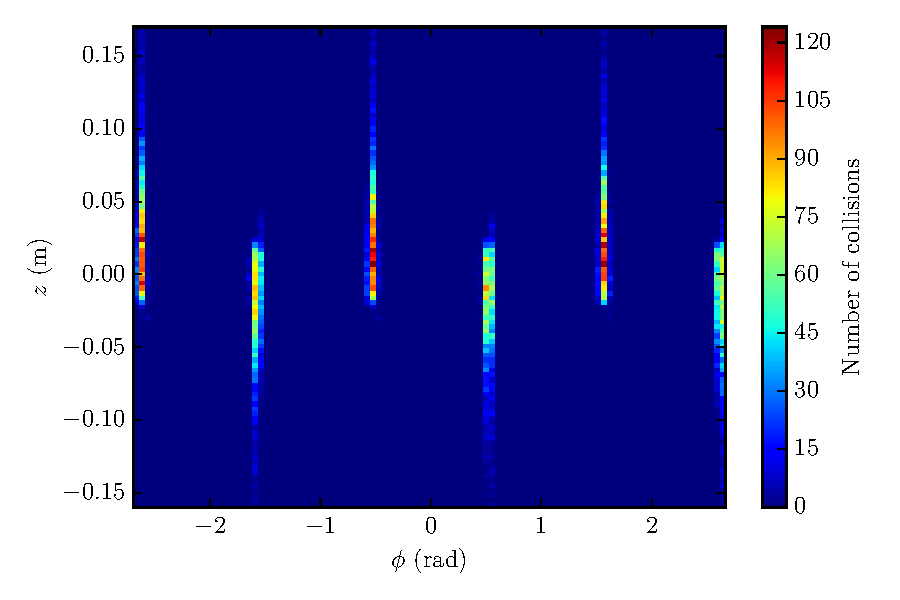
\includegraphics{output/cylinder_collision_points.pdf}
    \caption{Histogram of electron collision locations at the wall of the cylinder.}
    \label{fig:wall}
\end{figure}

In the absence of electric fields, the particles' kinetic energy should be conserved in this kind of a magnetic bottle. This was verified by calculating the mean and standard deviation of the final particle energies. The mean energy was $\langle E_\text{final} \rangle = 10000\,\si{\electronvolt}$ and the standard deviation $\sigma(E_\text{final}) \approx 0.012\,\si{\electronvolt}$, which very strictly equals to the initial $10\,\si{\kilo\electronvolt}$ energy given to the particles. It is concluded that energy is conserved in the simulation.

In the simulation, the radial and transverse components $(v_\parallel, v_\perp)$ of the particle starting velocities w.r.t. $\mathbf{B}$ field were logged. These are plotted in figure~\ref{fig:vel} separately for lost and non-lost particles. From there one can determine the limits of the loss cone angle.
\begin{figure}
    \centering
    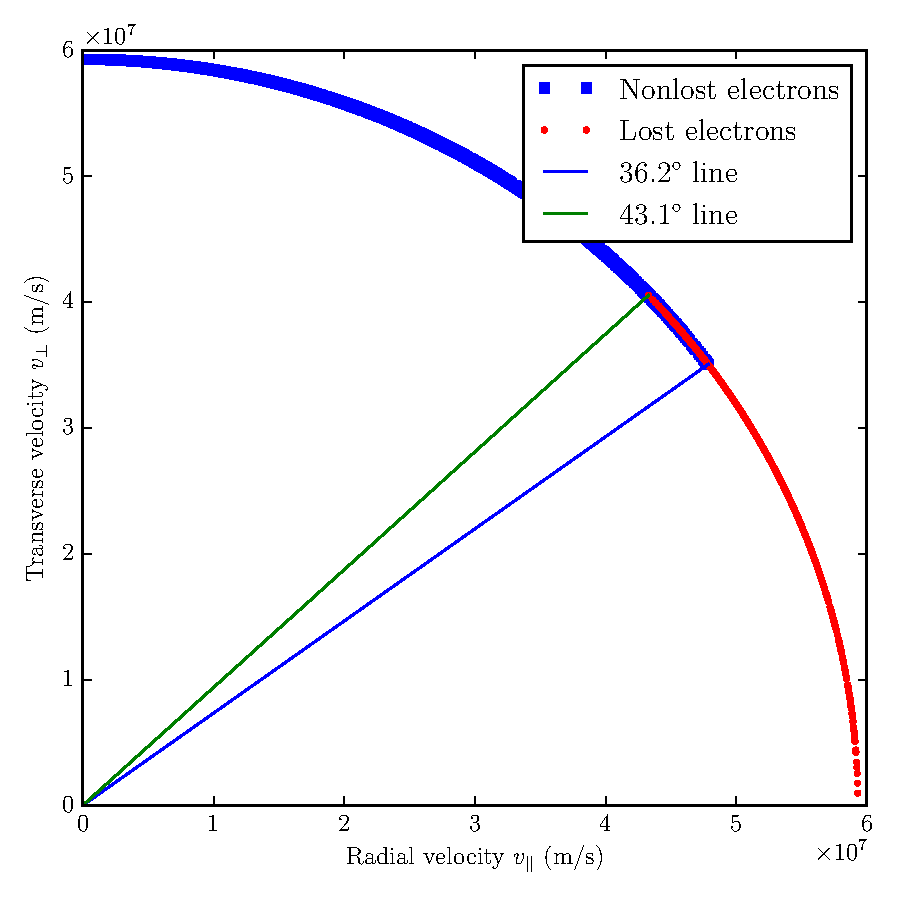
\includegraphics{output/loss_cone.pdf}
    \caption{Test particle initial velocities in $(v_\parallel, v_\perp)$ coordinates with respect to the direction of the initial magnetic $\mathbf{B}$ field.}
    \label{fig:vel}
\end{figure}
In this situation, one can't define a single loss cone angle as there are multiple different magnetic mirrors in the magnetic field configuration. Instead, limit angles of certain loss and confinement can be determined. The velocity data was analyzed programmatically, and it wass found that the maximal loss angle was $43.1\,\si{\degree}$ and the minimal confinement angle was $36.2\,\si{\degree}$. The theoretical expression for the loss cone angle of a magnetic mirror is
\begin{equation}
    \label{eq:losscone}
    \theta = \arcsin{\sqrt{\frac{B_0}{B_\text{max}}}},
\end{equation}
where $B_0$ is the magnitude of the magnetic field at the initial position of the electron and $B_\text{max}$ is the maximum of the magnetic field of a particular magnetic mirror.

For the ECR ion source in the simulation, $B_0$ is the value of the magnetic flux density at the ECR surface (that is, where the electrons are accelerated), in this case $B_0 = 0.5\,\si{\tesla}$. From figure~\ref{fig:solenoidb} two maxima are found: $B_\text{max,1} \approx 1.83\,\si{\tesla}$ on the left and $B_\text{max,2} \approx 1.05\,\si{\tesla}$ on the right. For these, one gets loss cone angles of $\theta_1 \approx 31.5\,\si{\degree}$ and $\theta_2 \approx 43.6\,\si{\degree}$. Here a clear correspondence between $\theta_2$ and the $43.1\,\si{\degree}$ maximal loss angle is found. This is a desirable result, since in a ECR ion source the magnetic mirror at the extraction end should dominate the loss cone angle, which happens here. Moreover, roughly $4.6\,\si{\percent}$ of all the lost particles hit the $z_1$ end and $14.3\,\si{\percent}$ hit the $z_2$ end i.e. the extraction. The rest of the particles were lost to the walls at the amount of $81.0\,\si{\percent}$ which seems quite high. Thus, the confinement at the sides of a cylindrical configuration is weaker.

\begin{thebibliography}{9}
    \bibitem{code}
        Simulation library: \url{https://yousource.it.jyu.fi/erkka/erkka/trees/master/app/plasma_physics_assignment} and control code: \url{https://yousource.it.jyu.fi/erkka/erkka/trees/master}. S. Kapanen, 2016.

    \bibitem{instr}
        Numerical exercise --- Electron in an ECRIS. T. Kalvas. JYFL, 2016.

    \bibitem{lecnotes}
        FYSS360 lecture notes. V. Toivanen, H. Pitkänen. JYFL, 2014.
\end{thebibliography}

\end{document}

